\documentclass[b5paper]{report}

\usepackage{graphicx}
\usepackage{mwe}

\usepackage{skeldoc}
\usepackage[kw]{pseudo}
\usepackage{tcolorbox}
\usepackage{tabto}

\definecolor{lighttan}{cmyk}{0,0.05,0.17,0}
\definecolor{darktan}{cmyk}{0,0.07,0.26,0.06}
\pseudoset{label=\small\arabic*, hd-space}

\usepackage{jlcode}

\usepackage{caption}
\usepackage{threeparttable}

\usepackage{amsmath}
\usepackage{amssymb}

\usepackage[page,toc,titletoc,title]{appendix}
\usepackage{hyperref}

\tcbuselibrary{skins,theorems}
\newtcbtheorem{algorithm}{Algorithm}{pseudo/boxruled, float}{alg}
% colback = lighttan, colbacktitle = darktan
\TabPositions{2cm}

\begin{document}

\newcommand{\mono}[1]{$\texttt{#1}$}

\begin{titlepage}
  \newcommand{\HRule}{\rule{\linewidth}{0.5mm}}

  \vbox{ }
  \vbox{ }
  \begin{center}
    % Upper part of the page
    
\includegraphics[width=0.15\textwidth]{ntnu.png}\\[1cm]
    \textsc{\Large Department of Computer Science}\\[1.5cm]
    \textsc{\large TDT4900 --- Master's thesis}\\[0.5cm]
    \vbox{ }

    % Title
    \HRule \\[0.4cm]
    { \huge \bfseries Matroids and fair allocation}\\[0.4cm]
    \HRule \\[1.5cm]

    % Author
    \large
    \emph{Author:}\\
    Andreas Aaberge Eide\\[0.5cm]
    \emph{Supervisor:}\\
    Magnus Lie Hetland
    \vfill

    % Bottom of the page
    {\large \today\par}
  \end{center}
\end{titlepage}

\tableofcontents

\chapter{Introduction}

Fair allocation is the problem of \textit{fairly} partitioning a set of resources among individuals with different preferences over these resources. This has been a hot topic of interest since antiquity (the 2000-year old Babylonian Talmud includes a discussion on how to distribute the estate of a deceased debtor among his creditors, for example~\cite{aumann-1985}), and remains so today. As societies are faced with rising economical and environmental pressures have to do more with less, the problem of achieving fair and efficient allocations will remain central. 

The mathematical study of fair allocation started with Hugo Steinhaus as late as 1948~\cite{steinhaus-1948}, and for decades the focus was largely on the \textit{divisible} case, in which the resources can be divided into arbitrary small pieces, and envy-free allocations (in which no agent values another agent's bundle higher than her own) always exist~\cite{amanatidis2022fair}. More recently, fair allocation of \textit{indivisible} goods has garnered the attention of computer scientists, who have brought algorithmic techniques to the field to great effect. 

\begin{enumerate}
  \item Computer science offers a fresh angle to further the research agenda for indivisible fair allocation
  \item EF, EFX, egalitarian welfare, Nash welfare -- all NP-hard...
  \item ...in the general, additive case. Reduced problem instances!
  \item Matroids are great, Yankee Swap is really fair...
  \subitem -- strong possibility results, polynomial-time computable
  \item ...but little tooling exists for empirical working
\end{enumerate}

One goal for this project is to create a library for the Julia programming language~\cite{bezanson2017julia}, supplying functionality for generating and interacting with (random) matroids. Throughout the text I will refer to this library as Matroids.jl. In the preparatory project delivered fall of 2022, I implemented Knuth's 1974 algorithm for the random generation of arbitrary matroids via the erection of closed sets \cite{knuth-1975}. With this, I was able to randomly generate matroids of universe sizes $n \leq 12$, but for larger values of $n$ my implementation was unbearably slow. 
\chapter{Background}

\section{Matroid theory}
\label{sec:matroid-theory}
If a mathematical structure can be defined or axiomatized in multiple different, but not obviously equivalent, ways, the different definitions or axiomatizations of that structure make up a cryptomorphism. The many obtusely equivalent definitions of a matroid are a classic example of cryptomorphism, and belie the fact that the matroid is a generalization of concepts in many, seemingly disparate areas of mathematics.

First introduced by Hassler Whitney in 1935~\cite{whitney-1935}, in a seminal paper where he described two axioms for independence in the columns of a matrix, and defined any system obeying these axioms to be a ``matroid''. Whitney's key insight was that this abstraction of~~``independence'' is applicable to both matrices and graphs. As a result of this, the terms used in matroid theory are borrowed from analogous concepts in both graph theory and linear algebra. Matroids have also received attention from researchers in fair allocation, as their properties make them useful for modeling user preferences; for instance, matroid rank functions are a natural way of formally describing course allocation for students~\cite{benabbou-2021}. 

\subsection*{Independent sets}
Perhaps the most common way to define a matroid is in terms of its \textit{independent sets}. An independence system is a pair $(E, \mathcal{I})$, where $E$ is the ground set of elements, $E \not= \emptyset$, and $\mathcal{I}$ is the set of independent sets, $\mathcal{I} \subseteq 2^E$. A matroid is an independence system with the following properties:

\begin{enumerate}
  \item The empty set is independent: $\emptyset \in \mathcal{I}$.
  \item The hereditary property: if $A \subseteq B$ and $B \in \mathcal{I}$, then $A \in \mathcal{I}$.
  \item The augmentation property: If $A, B \in \mathcal{I}$ and $|A| > |B|,$ then there exists $e \in A$ such that $B \cup \{e\} \in S$.
\end{enumerate}

In practice, the ground set $E$ represents the universe of elements in play, and the independent sets of typically represent the legal combinations of these items. In the context of fair allocation, the independent sets represent the legal (in the case of matroid constraints) or desired (in the case of matroid utilities) bundles of items.

\subsection*{Rank}
Given a matroid $\mathfrak{M} = (E, \mathcal{I})$, the \textit{matroid rank function} (MRF) is a function $\fn{rank} : 2^E \to \mathbb{Z}^+$ that gives the \textit{rank} of a set $ A \subseteq E$, which is defined to be the size of the largest independent subset of $A$. Formally, $$\fn{rank}(A) = \max\{|X| : X \subseteq A \text{ and } X \in \mathcal{I}\}.$$ Matroid rank functions are \textit{binary submodular}. Binary because they have binary marginals, that is, $\fn{rank}(A \cup \{ e \}) - \fn{rank}(A) \in \{0,1\}$, for all $A \subseteq 2^E$ and $e \in E$. Submodularity refers to rank functions' natural diminishing returns property, namely that for any two sets $X, Y \subseteq E$, we have $$\fn{rank}(X \cup Y) + \fn{rank}(X \cap Y) \leq \fn{rank}(X) + \fn{rank}(Y).$$ This diminishing returns property makes the rank function useful for modeling user preferences, and is a reason why matroids show up so often in economics and game theory (???).

\subsection*{Closed sets}

We also need to establish the concept of the \textit{closed sets} of a matroid. A closed set is a set whose cardinality is maximal for its rank. Equivalently to the definition given above, we can define a matroid as $\mathfrak{M} = (E, \mathcal{F})$, where $\mathcal{F}$ is the set of closed sets of $\mathfrak{M}$, satisfying the following properties:

\begin{enumerate}
  \item The set of all elements is closed: $E \in \mathcal{F}$
  \item The intersection of two closed sets is a closed set: If $A,B \in \mathcal{F},$ then $A \cap B \in \mathcal{F}$
  \item If $A \in \mathcal{F}$ and $a,b \in E \setminus A,$ then $b$ is a member of all sets in $\mathcal{F}$ containing $A \cup \{a\}$ if and only if $a$ is a member of all sets in $\mathcal{F}$ containing $A \cup \{b\}$
\end{enumerate}

\section{Examples of matroids}
\skelpar

\subsection*{The free matroid}
\skelpar

\subsection*{The uniform matroid}
\skelpar

\subsection*{The vector matroid}
\skelpars[2]

\subsection*{The graphic matroid}
\skelpars[3]
\chapter{Random matroid generation}

One goal for this project is to create the Julia library \mono{Matroids.jl}, which will supply functionality for generating and interacting with random matroids. In the preparatory project delivered fall of 2022, I implemented Knuth's 1974 algorithm for the random generation of arbitrary matroids via the erection of closed sets \cite{knuth-1975}. With this, I was able to randomly generate matroids of universe sizes $n \leq 12$, but for larger values of $n$ my implementation was unbearably slow. In this chapter, Knuth's method for random matroid construction will be described, along with the steps I have taken to speed up my initial, naïve implementation. The random generation of other specific types of matroids is discussed as well.

\section{Knuth's matroid construction (KMC)}
\pr{Knuth-Matroid} (given in Algorithm~\ref{alg:knuth}) accepts the ground set $E$ and a list of enlargements $\mathrm{X}$, and produces the matroid $\mathfrak{M} = (E, \mathcal{F})$, such that for each set $X \in \mathrm{X}[r]$, we have $X \in \mathcal{F}, \text{ rank}(X) = r$. The algorithm outputs the tuple $(E, \mathrm{F})$, where $\mathrm{F} = [F_0, \ldots, F_r]$, $r$ being the final rank of $\mathfrak{M}$ and $F_i$ the family of closed sets of rank $i$. In the paper, Knuth shows that $\bigcup_{i=0}^r \mathrm{F}[r] = \mathcal{F}$, and so the algorithm produces a valid matroid represented by its closed sets.

The \textit{covers} of a closed set $A$ of rank $r$ are the sets obtained by adding one more element from $E$ to $A$. The algorithm proceeds in a bottom-up manner, starting with the single closed set of rank 0 (the empty set) and for each rank $r+1$ adds the covers of the closed sets of rank $r$. The covers are generated with the helper method \pr{Generate-Covers}(\mathrm{F}, r, E).

\begin{tcolorbox}[pseudo/boxruled]
  \begin{pseudo}*
    \hd{Generate-Covers}(\mathrm{F}, r, E) \\
    return $\{ A \cup \{a\} : A \in \mathrm{F}[r], a \in E \setminus A \}$
  \end{pseudo}
\end{tcolorbox}

Given no enlargements ($\mathrm{X} = []$), the resulting matroid is the free matroid over $E$. Arbitrary matroids can be generated by supplying different lists $\mathrm{X}$. When enlarging, the sets in $\mathrm{X}[r+1]$ are simply added to $\mathrm{F}[r+1]$.

\pr{Superpose!}(\mathrm{F}[r+1], F[r]) ensures that the newly enlarged family of closed sets of rank $r+1$ is valid. If $F_{r+1}$ contains two sets $A,B$ whose intersection $A \cap B \not \subseteq C$ for any $C \in F_{r}$, replace $A,B$ with $A \cup B$. Repeat until no two sets exist in $F_{r+1}$ whose intersection is not contained within some set $C \in F_{r}$.

\begin{tcolorbox}[pseudo/boxruled, float*=ht!]
  \begin{pseudo}[kw, indent-mark]*
    \hd{Superpose!}({F_{r+1},F_r}) \\
    for $A \in F_{r+1}$ \\+
    for $B \in F_{r+1}$ \\+
    \id{flag} $\leftarrow$ \cn{true} \\
    for $C \in F_r$ \\+
    if $A \cap B \subseteq C$ \\+
    \id{flag} $\leftarrow$ \cn{false} \\--
    \\
    if \id{flag} = \cn{true} \\+
    $F_{r+1} \leftarrow F_{r+1} \setminus \{A, B \}$ \\
    $F_{r+1} \leftarrow F_{r+1} \cup \{A \cup B \}$
  \end{pseudo}
\end{tcolorbox}

\begin{algorithm}[float*=ht!]{\pr{Knuth-Matroid}(E, \mathrm{X})}{knuth}

  \textbf{Input:}     \tab The ground set of elements $E$, and a list of enlargements $\mathrm{X}$.

  \textbf{Output:}    \tab The list of closed sets of the resulting matroid grouped by rank, \\
  \mbox{}\tab $\mathrm{F} = [F_0, \ldots, F_r]$, where $F_i$ is the set of closed sets of rank $i$.

  \begin{pseudo}[kw, label=\small\arabic*, indent-mark, line-height=1.2]
    $r = 0, \mathrm{F} = [\{ \emptyset \}]$ \\
    while \cn{true}  \\+
    $\pr{Push!}(\mathrm{F}, \pr{Generate-Covers}(\mathrm{F}, r, E))$ \\
    $\mathrm{F}[r+1] = \mathrm{F}[r+1] \cup \mathrm{X}[r+1]$ \\
    \pr{Superpose!}(\mathrm{F}[r+1], \mathrm{F}[r]) \\

    if $E \not \in F[r+1]$ \\+
    $r \leftarrow r+1$ \\-
    else \\+
    return $(E, \mathrm{F})$

  \end{pseudo}

\end{algorithm}


\subsection{Randomized KMC}
In the randomized version of \pr{Knuth-Matroid}, we generate matroids by applying a supplied number of random coarsening steps, instead of enlarging with supplied sets. This is done by applying \pr{Superpose!} immediately after adding the covers, then choosing a random member $A$ of $\mathrm{F}[r+1]$ and a random element $a \in E \setminus A$, replacing $A$ with $A \cup \{a\}$ and finally reapplying \pr{Superpose!}. The parameter $p = (p_1, p_2, \ldots)$ gives the number of such coarsening steps to be applied at each iteration of the algorithm.

The pseudocode given up to this point corresponds closely to the initial Julia implementation, which can be found in Appendix~\ref{apx:randkmcv1}. It should already be clear that this brute force implementation leads to poor performance -- for instance, the \pr{Superpose!} method uses a triply nested for loop, which should be a candidate for significant improvement if possible. Section~\ref{sec:improving-performance} describes the engineering work done to create a more performant implementation.

\begin{algorithm}[float*=ht!]{\pr{Randomized-Knuth-Matroid}(E, p)}{rkmc}

  \textbf{Input:}     \tab The ground set of elements $E$, and a list $p = [p_1, p_2, ...]$, where \\
  \mbox{}\tab $p_r$ is the number of coarsening steps to apply at rank $r$ in the \\
  \mbox{}\tab construction.

  \textbf{Output:}    \tab The list of closed sets of the resulting matroid grouped by rank, \\
  \mbox{}\tab $\mathrm{F} = [F_0, \ldots, F_r]$, where $F_i$ is the set of closed sets of rank $i$.

  \begin{pseudo}[label=\small\arabic*, indent-mark, line-height=1.2]
    $r = 0, \mathrm{F} = [\{ \emptyset \}]$ \\
    \kw{while} \cn{true}  \\+
      $\pr{Push!}(\mathrm{F}, \pr{Generate-Covers}(\mathrm{F}, r, E))$ \\
      \pr{Superpose!}(\mathrm{F}[r+1], \mathrm{F}[r]) \\
      
      \kw{if} $E \in \mathrm{F}[r+1]$ \kw{return} $(E, \mathrm{F})$ \\
      
      \kw{while} $p[r] > 0$ \\+
        $A \leftarrow$ a random set in $\mathrm{F}[r+1]$ \\
        $a \leftarrow$ a random element in $E \setminus A$ \\
        \kw{replace} $A$ with $A \cup \{a\}$ in $\mathrm{F}[r+1]$ \\
        \pr{Superpose!}(\mathrm{F}[r+1], \mathrm{F}[r]) \\

        \kw{if} $E \in \mathrm{F}[r+1]$ \kw{return} $(E, \mathrm{F})$ \\

        $p[r] = p[r] - 1$ \\-
      $r = r + 1$

  \end{pseudo}

\end{algorithm}


\subsection{Improving performance}
\label{sec:improving-performance}
When recreating Knuth's table of observed mean values for the randomly generated matroids, some of the latter configurations of $n$ and $(p_1, p_2, \ldots)$ was unworkably slow, presumably due to my naïve implementation of the algorithm. Table~\ref{tab:perf_v1} shows the performance of this first implementation.

\begin{table*}[ht!]
  \centering
  \caption{Performance of $\texttt{random\_kmc\_v1}$.}
  \label{tab:perf_v1}
  \begin{threeparttable}
    \begin{tabular}{llllllllll}
      \toprule
      $n$ & $(p_1, p_2, \ldots)$ & Trials & Time  & GC Time & Bytes allocated \\
      \midrule
        10 & (0, 6, 0)    & 100 & 0.0689663   & 0.0106786 & 147.237 MiB \\
        10 & (0, 5, 1)    & 100 & 0.1197194   & 0.0170734 & 251.144 MiB \\
        10 & (0, 5, 2)    & 100 & 0.0931822   & 0.0144022 & 203.831 MiB \\
        10 & (0, 6, 1)    & 100 & 0.0597314   & 0.0094902 & 132.460 MiB \\
        10 & (0, 4, 2)    & 100 & 0.1924601   & 0.0284532 & 406.131 MiB \\
        10 & (0, 3, 3)    & 100 & 0.3196838   & 0.0463972 & 678.206 MiB \\
        10 & (0, 0, 6)    & 100 & 1.1420602   & 0.1671325 & 2.356 GiB   \\
        10 & (0, 1, 1, 1) & 100 & 2.9283978   & 0.3569357 & 5.250 GiB   \\
        13 & (0, 6, 0)    & 10  & 104.0171128 & 9.9214449 & 161.523 GiB \\
        13 & (0, 6, 2)    & 10  & 11.4881308  & 1.3777947 & 20.888 GiB  \\
        16 & (6, 0, 0)    & 1   & -           & -         & -           \\
      \bottomrule
    \end{tabular}
  \end{threeparttable}
\end{table*}

The performance was measured using Julia's \jlinl{@timed}\footnote{\href{https://docs.julialang.org/en/v1/base/base/\#Base.@timed}{https://docs.julialang.org/en/v1/base/base/\#Base.@timed}} macro, which returns the time it takes to execute a function call, how much of that time was spent in garbage collection and the number of bytes allocated. As is evident from the data, larger matroids are computationally quite demanding to compute with the current approach, and the time and space requirements scales exponentially with $n$. Can we do better? As it turns out, we can; after the improvements outlined in this section, we will be able to generate matroids over universes as large as $n=128$ in a manner of seconds and megabytes.

\subsubsection{Representing sets as binary numbers}
The first improvement we will attempt is to represent our closed sets using one of Julia's \jlinl{Integer} types of bit width at least $n$, instead of as a \jlinl{Set}\footnote{\href{https://docs.julialang.org/en/v1/base/collections/\#Base.Set}{https://docs.julialang.org/en/v1/base/collections/\#Base.Set}} of elements of $E$. Appendix~\ref{apx:code} contains all the code referenced in this chapter; the Julia implementation at this point can be found in \ref{apx:randkmcv2}. 

\skelpar{Skrive mer om hvordan Set\{Set\{Integer\}\} lagres i minnet og fordelene med å gå over til Set\{Integer\}.}

The idea is to define a family of closed sets of the same rank as \jlinl{Set\{UInt16\}}. Using \jlinl{UInt16} we can support ground sets of size up to 16. Each 16-bit number represents a set in the family. For example, the set $\{ 2,5,7 \}$ is represented by $$164 = 0\rm{x}00\rm{a}4 = 0\rm{b}0000000010100100 = 2^7+2^5+2^2.$$ At either end we have $\emptyset \equiv 0\rm{x}0000$ and $E \equiv 0\rm{xffff}$ (if $n = 16$). The elementary set operations we will need have simple implementations using bitwise operations.

\begin{table}[!ht]
  % \caption{Set operations and their equivalent bitwise operations}
  \centering
  \begin{tabular}{|l|l|}
  \hline
      Set operation & Bitwise operation \\\hline
      $A \cap B$      & $A$ AND $B$ \\\hline
      $A \cup B$      & $A$ OR $B$ \\\hline
      $A \setminus B$ & $A$ AND NOT $B$ \\\hline
      $A \subseteq B$ & $A$ AND $B$ = $A$ \\\hline
  \end{tabular}
\end{table}

We can now describe the bitwise versions of the required methods. The bitwise implementation of \pr{Generate-Covers} finds all elements in $E \setminus A$ by finding each value $0\leq i< n$ for which \jlinl{A & 1 << i === 0}, meaning that the set represented by \jlinl{1 << i} is not a subset of A. The bitwise implementation of \pr{Superpose!} is unchanged apart from using the bitwise set operations described above.

\begin{table*}[ht!]
  \centering
  \caption{Performance of $\texttt{random\_kmc\_v2}$.}
  \label{tab:perf_v2}
  \begin{threeparttable}
    \begin{tabular}{llllllllll}
      \toprule
      $n$ & $(p_1, p_2, \ldots)$ & Trials & Time  & GC Time & Bytes allocated \\
      \midrule
      10 & [0, 6, 0] & 100 & 0.0010723 & 0.0001252 & 1.998 MiB \\ 
      10 & [0, 5, 1] & 100 & 0.0017543 & 0.0001431 & 3.074 MiB \\ 
      10 & [0, 5, 2] & 100 & 0.0008836 & 0.0001075 & 2.072 MiB \\ 
      10 & [0, 6, 1] & 100 & 0.0007294 & 6.73e-5 & 1.700 MiB \\ 
      10 & [0, 4, 2] & 100 & 0.0020909 & 0.0001558 & 3.889 MiB \\ 
      10 & [0, 3, 3] & 100 & 0.0024636 & 0.0002139 & 4.530 MiB \\ 
      10 & [0, 0, 6] & 100 & 0.007082 & 0.0004801 & 9.314 MiB \\ 
      10 & [0, 1, 1, 1] & 100 & 0.0132477 & 0.0008307 & 17.806 MiB \\ 
      13 & [0, 6, 0] & 10 & 0.042543 & 0.0014988 & 31.964 MiB \\ 
      13 & [0, 6, 2] & 10 & 0.0183313 & 0.0012176 & 21.062 MiB \\ 
      16 & [0, 6, 0] & 10 & 1.2102877 & 0.0146129 & 450.052 MiB \\ 
      \bottomrule
    \end{tabular}
  \end{threeparttable}
\end{table*}

The performance of \mono{random\_kmc\_v2} is shown in Table~\ref{tab:perf_v2}. It is clear that representing closed sets using binary numbers represents a substantial improvement -- we are looking at performance increases of 100x-1000x across the board. Great stuff!


\subsubsection{Sorted superpose}
Can we improve the running time of the algorithm further? It is clear that \pr{Superpose!} takes up a large portion of the compute time. In the worst case, when no enlargements have been made, $F_{r+1}$ is the set of all $r+1$-sized subsets of $E$, $|F_{r+1}| = {\binom{n}{r+1}}$. Comparing each $A,B \in F_{r+1}$ with each $C \in F_r$ in a triply nested for loop requires $\mathcal{O}({\binom{n}{r+1}}^2{\binom{n}{r}})$ operations. In the worst case, no enlargements are made at all, and we build the free matroid in $\mathcal{O}(2^{3n})$ time (considering only the superpose step).

After larger closed sets have been added to $\mathrm{F}[r+1]$, \pr{Superpose!} will cause sets to merge, so that only maximal dependent sets remain. Some sets will even simply disappear. In the case where $X=\{1,2\}$ was added by \pr{Generate-Covers}, and the $Y=\{1,2,3\}$ was added manually as an enlargement, the smaller set will be fully subsumed in the bigger set, as $\{1,2\}\cap\{1,2,3\}=\{1,2\}$ (which is not a subset of any set in $\mathrm{F}[r]$) and $\{1,2\}\cup\{1,2,3\}=\{1,2,3\}$. In this situation, $Y$ would ``eat'' the covers $\{1,3\}$ and $\{2,3\}$ as well. This fact is reflected in the performance data -- notice how much more space is demanded by the 10-element matroid with $p=[0,0,6]$ than the one with $p=[0,6,0]$ in any of the performance tables in this section. Making enlargements at earlier ranks will result in smaller matroids as more sets will get absorbed.

\begin{jllisting}
function sorted_bitwise_superpose!(F, F_prev)
  As = sort!(collect(F), by = s -> length(bits_to_set(s)))
  while length(As) !== 0
    A = popfirst!(As)

    for B in setdiff(F, A)
      if should_merge(A, B, F_prev)
        insert!(As, 1, A | B)
        setdiff!(F, [A, B])
        push!(F, A | B)
        break
      end
    end
  end

  return F
end
\end{jllisting}

Since the larger sets will absorb so many of the smaller sets (around $\binom{p}{r+1}$, where $p$ is the size of the larger set and $r+1$ is the size of the smallest sets allowed to be added in a given iteration), might it be an idea to perform the superpose operation in descending order based on the size of the sets? This should result in fewer calls to \pr{Superpose!}, as the bigger sets will remove the smaller sets that fully overlap with them in the early iterations, however, the repeated sorting of the sets might negate this performance gain. This is the idea behind \jlinl{sorted_bitwise_superpose!}, which was used in \jlinl{random_kmc_v3}. The full code can be found in Appendix~\ref{apx:randkmcv2}.

Unfortunately, as Table~\ref{tab:perf_v3} shows, this implementation is a few times slower and more space demanding than the previous implementation. This is might be due to the fact that an ordered list is more space inefficient than the hashmap-based \jlinl{Set}.

\begin{table*}[ht!]
  \centering
  \caption{Performance of $\texttt{random\_kmc\_v3}$.}
  \label{tab:perf_v3}
  \begin{threeparttable}
    \begin{tabular}{llllllllll}
      \toprule
      $n$ & $(p_1, p_2, \ldots)$ & Trials & Time  & GC Time & Bytes allocated \\
      \midrule
      10 & [0, 6, 0] & 100 & 0.0023382 & 0.0001494 & 4.042 MiB \\
      10 & [0, 5, 1] & 100 & 0.001853 & 0.0001433 & 4.383 MiB \\
      10 & [0, 5, 2] & 100 & 0.0017845 & 0.0001341 & 4.043 MiB \\
      10 & [0, 6, 1] & 100 & 0.0015145 & 0.0001117 & 3.397 MiB \\
      10 & [0, 4, 2] & 100 & 0.0030704 & 0.0002125 & 6.385 MiB \\
      10 & [0, 3, 3] & 100 & 0.0037838 & 0.0002514 & 7.018 MiB \\
      10 & [0, 0, 6] & 100 & 0.008903 & 0.000557 & 14.159 MiB \\
      10 & [0, 1, 1, 1] & 100 & 0.0142828 & 0.0008823 & 21.838 MiB \\
      13 & [0, 6, 0] & 10 & 0.0627633 & 0.002094 & 51.492 MiB \\
      13 & [0, 6, 2] & 10 & 0.0106478 & 0.0007704 & 20.774 MiB \\
      16 & [0, 6, 0] & 10 & 0.6070136 & 0.0095656 & 310.183 MiB \\
      \bottomrule
    \end{tabular}
  \end{threeparttable}
\end{table*}


\subsubsection{Iterative superpose}
The worst-case $\mathcal{O}({\binom{n}{r+1}}^2{\binom{n}{r}})$ runtime of \pr{Superpose!} at step $r$ is due to the fact that it takes in $\mathrm{F}$ after all covers and enlargements have been indiscriminately added to $\mathrm{F}[r+1]$ and then loops through to perform the superposition. Might there be something to gain by inserting new closed sets into the current family one at a time, and superposing on the fly?
\pagebreak
\begin{jllisting}
  # Superpose (random_kmc_v4)
  push!(F, Set()) # Add F[r+1].
  while length(to_insert) > 0
    A = pop!(to_insert)
    push!(F[r+1], A)

    for B in setdiff(F[r+1], A)
      if should_merge(A, B, F[r])
        push!(to_insert, A | B)
        setdiff!(F[r+1], [A, B])
        push!(F[r+1], A | B)
      end
    end
  end
\end{jllisting}

In \jlinl{random_kmc_v4}, the full code of which can be found in Appendix~\ref{apx:randkmcv4}, the covers and enlargements are not added directly to $\mathrm{F}[r+1]$, but to a temporary array \jlinl{to_insert}. Each set $A$ is then popped from \jlinl{to_insert} one at a time, added to $\mathrm{F}[r+1]$ and compared with the other sets $B \in \mathrm{F}[r+1] \setminus \{A\}$ and $C \in \mathrm{F}[r]$ in the usual \pr{Superpose!} manner. This results in fewer comparisons, as each set is only compared with the sets added before it; the first set is compared with no other sets, the second set with one other and the sets in $\mathrm{F}[r]$, and so on. The number of such comparisons is therefore given by the triangular number $T_{\binom{n}{r+1}}$, and so we should have roughly halved the runtime at step $r$. It is worth noting that this implementation of \pr{Superpose!} uses a subroutine \jlinl{should_merge} that returns early when it finds one set $C \in \mathrm{F}[r]$ such that $C \supseteq A \cap B$, so in practice it usually does not require $\binom{n}{r}$ comparisons in the innermost loop.

Table~\ref{tab:perf_v4} shows that the iterative superpose was a meaningful improvement. For most input configurations, it is a few times faster and a few times less space demanding than \jlinl{random_kmc_v2}.


\begin{table*}[ht!]
  \centering
  \caption{Performance of $\texttt{random\_kmc\_v4}$.}
  \label{tab:perf_v4}
  \begin{threeparttable}
    \begin{tabular}{llllllllll}
      \toprule
      $n$ & $(p_1, p_2, \ldots)$ & Trials & Time  & GC Time & Bytes allocated \\
      \midrule
      10 & [0, 6, 0]    & 100 & 0.0014585  & 3.94e-5   & 724.635 KiB \\ 
      10 & [0, 5, 1]    & 100 & 0.0007192  & 9.39e-5   & 659.729 KiB \\ 
      10 & [0, 5, 2]    & 100 & 0.0005943  & 3.53e-5   & 617.668 KiB \\ 
      10 & [0, 6, 1]    & 100 & 0.0003502  & 2.88e-5   & 408.666 KiB \\ 
      10 & [0, 4, 2]    & 100 & 0.001013   & 5.36e-5   & 887.618 KiB \\ 
      10 & [0, 3, 3]    & 100 & 0.0011847  & 5.03e-5   & 1.003 MiB   \\ 
      10 & [0, 0, 6]    & 100 & 0.0015756  & 9.7e-5    & 1.066 MiB   \\ 
      10 & [0, 1, 1, 1] & 100 & 0.0046692  & 0.0001385 & 2.455 MiB   \\ 
      13 & [0, 6, 0]    & 10  & 0.0118201  & 0.0005486 & 6.289 MiB   \\ 
      13 & [0, 6, 2]    & 10  & 0.0075668  & 0.0002458 & 4.666 MiB   \\ 
      16 & [0, 6, 0]    & 10  & 0.2819294  & 0.0040792 & 81.317 MiB  \\ 
      16 & [0, 6, 1]    & 10  & 0.8268207  & 0.0070206 & 154.451 MiB \\ 
      16 & [0, 0, 6]    & 10  & 95.1959596 & 0.0290183 & 553.597 MiB \\ 
      \bottomrule
    \end{tabular}
  \end{threeparttable}
\end{table*}

\subsubsection{Rank table}
While \pr{Superpose!} is getting more efficient, it is still performing the same comparisons over and over again. Let's consider what we are really trying to achieve with this function, to see if we can't find a smarter way to go about it.

After adding the closed sets for a rank, \pr{Superpose!} is run to maintain the closed set properties of the matroid (given in Section~\ref{sec:matroid-theory}). These are maintained by ensuring that, for any two newly added sets $A,B \in \mathrm{F}[r+1]$, there exists $C \in \mathrm{F}[r]$ such that $A \cap B \subseteq C$. Until this point, this has been done by checking if the intersection of each such $A,B$ is contained in a set $C$ of rank $r$. We remember that one of the properties of the closed sets of a matroid is that the intersection of two closed sets is itself a closed set. Therefore, we do not need to find a closed set $C$ that \textit{contains} $A \cap B$, since if $A$ and $B$ are indeed closed sets, their intersection will be \textit{equal} to some closed set $C$ of lesser rank. This insight leads us to the next improvement: if we keep track of all added closed sets in a rank table, then we can memoize \pr{Superpose!} and replace the innermost loop with a constant time dictionary lookup.

\begin{jllisting}
  # The rank table maps from the representation of a set to its assigned rank.
  rank = Dict{T, UInt8}(0=>0)
  
  [...]
  
  # Superpose.
  push!(F, Set()) # Add F[r+1].
  while length(to_insert) > 0
    A = pop!(to_insert)
    push!(F[r+1], A)
    rank[A] = r
  
    
    for B in setdiff(F[r+1], A)
      if !haskey(rank, A&B) || rank[A&B] >= r
        # Update insert queue.
        push!(to_insert, A | B)
    
        # Update F[r+1].
        setdiff!(F[r+1], [A, B])
        push!(F[r+1], A | B)
    
        # Update rank table.
        rank[A|B] = r
        break
      end
    end
  end
\end{jllisting}
\begin{table*}[ht!]
  \centering
  \caption{Performance of $\texttt{random\_kmc\_v5}$.}
  \label{tab:perf_v5}
  \begin{threeparttable}
    \begin{tabular}{llllllllll}
      \toprule
      $n$ & $(p_1, p_2, \ldots)$ & Trials & Time  & GC Time & Bytes allocated \\
      \midrule
      10 & [0, 6, 0] & 100 & 0.0001335 & 0.0 & 138.966 KiB \\
      10 & [0, 5, 1] & 100 & 0.0001436 & 0.0 & 158.691 KiB \\
      10 & [0, 5, 2] & 100 & 0.0001928 & 0.0 & 167.487 KiB \\
      10 & [0, 6, 1] & 100 & 0.0002204 & 0.0 & 148.812 KiB \\
      10 & [0, 4, 2] & 100 & 0.0001578 & 0.0 & 173.455 KiB \\
      10 & [0, 3, 3] & 100 & 0.0001743 & 0.0 & 202.566 KiB \\
      10 & [0, 0, 6] & 100 & 0.0003433 & 0.0 & 431.089 KiB \\
      10 & [0, 1, 1, 1] & 100 & 0.0004987 & 0.0 & 439.511 KiB \\
      13 & [0, 6, 0] & 100 & 0.0004776 & 0.0 & 422.431 KiB \\
      13 & [0, 6, 2] & 100 & 0.0003469 & 0.0 & 441.621 KiB \\
      16 & [0, 6, 0] & 100 & 0.0009073 & 0.0 & 1010.452 KiB \\
      16 & [0, 6, 1] & 100 & 0.0007939 & 0.0 & 997.022 KiB \\
      16 & [0, 0, 6] & 100 & 0.0066951 & 0.0 & 8.564 MiB \\
      20 & [0, 6, 0] & 100 & 0.0030797 & 0.0 & 4.042 MiB  \\
      20 & [0, 6, 2] & 10 & 0.0022849 & 0.0 & 4.547 MiB  \\
      32 & [0, 6, 2, 1] & 10 & 0.0269912 & 0.0 & 63.082 MiB  \\
      \bottomrule
    \end{tabular}
  \end{threeparttable}
\end{table*}
The full code for \jlinl{random_kmc_v5} can be found in Appendix~\ref{apx:randkmcv5}. Table~\ref{tab:perf_v5} shows that implementing a rank table was an extremely significant improvement. For smaller matroids, it is around 5-10x faster, however it is for larger matroids that it truly outshines its predecessors -- \jlinl{random_kmc_v5} is a whopping 13~000 times faster than \jlinl{random_kmc_v4} with $n=16, p=[0,0,6]$ as input.


\subsubsection{Non-redundant cover generation}
Up to this point, our cover generation routine has not taken into account that any two sets of rank $r$ will have at least one cover in common. To see this, consider a matroid-under-construction with $n=10$ where $A = \{1,2\}$ and $B = \{1,3\}$ are closed sets of rank 2. Currently, \pr{Generate-Covers} will happily generate the cover $C=\{1,2,3\}$ twice, once as the cover of $A$ and subsequently as the cover of $B$. Throughout this analysis, we will assume the worst case scenario of no enlargements, as any enlargements will strictly lower the number of sets in play at a given rank. In this case, $|\mathrm{F}[r]| = \binom{n}{r}$, and for each closed set $A$ of rank $r$ we are generating $|E\setminus A| = (n-r)$ covers, giving us a total of $\binom{n}{r}(n-r)$ covers generated at each rank $r$, including the duplicates. With no enlargements, we know that there are $\binom{n}{r+1}$ covers, and

$$\begin{aligned}
  (n-r)\binom{n}{r} &= \frac{n!(n-r)}{r!(n-r)!} \\
                    &= \frac{n!}{r!(n-r-1)!} \\
                    &= (r+1)\frac{n!}{(r+1)!(n-r-1)!} \\
                    &= (r+1)\binom{n}{r+1}. \\
\end{aligned}$$
For each step $r$, we are generating $r+1$ times as many covers as we need to. Over the course of all steps $0\leq r\leq n$, we are generating $$\sum_{r=0}^n (r+1) = \sum_{r=1}^{n+1}r = T_{n+1}$$ times the actual number of covers, where $T_{n+1}=\frac{(n+1)(n+2)}{2}$ is the triangular number. In other words, if we find a way to generate each cover only once, we will have shaved off an $n^2$ factor from the asymptotic complexity of our implementation.

When generating covers, \jlinl{random_kmc_v6} improves upon the brute force cover generation described above by only adding the covers 
$$\Bigl\{ A \cup \{ a \} : A \in \mathrm{F}[r], a \in E \setminus A, a \notin \bigcup \bigl\{ B : B \in \mathrm{F}[r+1], A \subseteq B \bigr\} \Bigr\}.$$
In other words, we find the covers of $A$, that is, the sets obtained by adding one more element $a$ from $E$ to $A$, but we do not include any $a$ that is to be found in another, already added, cover $B$ that contains $A$. This solves the problem described above; the cover $\{1,2,3\} = B \cup \{ 2 \}$ will not be generated, as $2 \in C$ and $B \subseteq C$. This is implemented in the following manner:

\begin{jllisting}
  # Generate minimal closed sets for rank r+1 (random_kmc_v6)
  for y in F[r] # y is a closed set of rank r.
    t = E - y # The set of elements not in y.
    # Find all sets in F[r+1] that already contain y and remove excess elements from t.
    for x in F[r+1]
      if (x & y == y) t &= ~x end
      if t == 0 break end
    end
    # Insert y ∪ a for all a ∈ t.
    while t > 0
      x = y|(t&-t)
      add_set!(x, F, r, rank)
      t &= ~x
    end
  end
\end{jllisting}
We have extracted the iterative superpose logic described above into its own function to allow it to be performed on a cover-per-cover basis:
\begin{jllisting}
function add_set!(x, F, r, rank)
  if x in F[r+1] return end
  for y in F[r+1]
    if haskey(rank, x&y) && rank[x&y]<r
    continue
    end
    
    # x ∩ y has rank > r, replace with x ∪ y.
    setdiff!(F[r+1], y)
    return add_set!(x|y, F, r, rank)
  end
  
  push!(F[r+1], x)
  rank[x] = r
end
\end{jllisting}
As such, $\mathrm{F}[r+1]$ is empty when the first cover $y \in \mathrm{F}$ is generated, and all covers $\{y \cup \{a\} : a \in E \setminus y\}$ are added. For later sets $y$, we are comparing with the previously added covers, and dropping any element to be found in a cover $x$ that fully includes $y$. This way, we avoid re-generating the cover $x$.


The full code for \jlinl{random_kmc_v6} can be found in Appendix~\ref{apx:randkmcv6}.

\begin{table*}[ht!]
  \centering
  \caption{Performance of $\texttt{random\_kmc\_v6}$.}
  \label{tab:perf_v6}
  \begin{threeparttable}
    \begin{tabular}{llllllllll}
      \toprule
      $n$ & $(p_1, p_2, \ldots)$ & Trials & Time  & GC Time & Bytes allocated \\
      \midrule
      10 & [0, 6, 0] & 100 & 0.000157 & 0.0 & 11.306 KiB \\
      10 & [0, 5, 1] & 100 & 0.0001427 & 0.0 & 12.257 KiB \\
      10 & [0, 5, 2] & 100 & 0.000121 & 0.0 & 11.568 KiB \\
      10 & [0, 6, 1] & 100 & 8.61e-5 & 0.0 & 10.447 KiB \\
      10 & [0, 4, 2] & 100 & 0.0001237 & 0.0 & 13.597 KiB \\
      10 & [0, 3, 3] & 100 & 0.0001233 & 0.0 & 14.029 KiB \\
      10 & [0, 0, 6] & 100 & 0.0002856 & 0.0 & 15.414 KiB \\
      10 & [0, 1, 1, 1] & 100 & 0.0001942 & 0.0 & 14.446 KiB \\
      13 & [0, 6, 0] & 100 & 0.0004483 & 0.0 & 19.117 KiB \\
      13 & [0, 6, 2] & 100 & 0.0004541 & 0.0 & 18.957 KiB \\
      16 & [0, 6, 0] & 10 & 0.0014919 & 0.0 & 34.531 KiB \\
      16 & [0, 6, 1] & 10 & 0.0014731 & 0.0 & 36.016 KiB \\
      16 & [0, 0, 6] & 10 & 0.0168858 & 0.0 & 127.652 KiB \\
      20 & [0, 6, 0] & 10 & 0.0061574 & 0.0 & 81.573 KiB \\
      20 & [0, 6, 2] & 10 & 0.0059717 & 0.0 & 82.323 KiB \\
      32 & [0, 6, 2, 1] & 10 & 0.1599507 & 0.0 & 279.531 KiB \\
      63 & [0, 6, 4, 2, 1] & 1 & 11.138914 & 0.0 & 4.912 MiB \\
      64 & [0, 6, 4, 4, 2, 1] & 1 & 12.508729 & 0.0 & 4.912 MiB \\
      128 & [0, 6, 6, 4, 4, 2, 1] & 1 & 1232.8570 & 0.0114583 & 102.159 MiB \\
      \bottomrule
    \end{tabular}
  \end{threeparttable}
\end{table*}
\skelpars[7]

\subsection{What do the generated matroids look like?}
\subsubsection{Observations}
\begin{enumerate}
  \item The average cardinality of the closed sets of a given rank is usually not very much higher than the rank. If the average cardinality were to stray much, all the sets merge instead and the sole closed set of that rank would become $E$. This might be a useful heuristic when finding the rank of a set.
\end{enumerate}

\skelpars[4]{@Benchmarking. Histogrammer. Beskrive variansen i matroide-størrelse ifht input.}

\subsection{Producing the rank function and independent sets}
To build a general matroid library, we want to be able to access all properties of a generated matroid $\mathfrak{M}$. This would include:
\begin{enumerate}
  \item the bases $\mathcal{B}$ of $\mathfrak{M}$,
  \item the independent sets $\mathcal{I}$ of $\mathfrak{M}$,
  \item the circuits $\mathcal{C}$ of $\mathfrak{M}$,
  \item the closure function $\fn{cl} : 2^E \to \mathcal{F}$, and
  \item the rank function $\fn{rank} : 2^E \to \mathbb{Z}^*$ of $\mathfrak{M}$.
\end{enumerate}

In this section, I will first describe an extension of \pr{Knuth-Matroid} that is also fully enumerates $\mathcal{I}$ and $\mathcal{C}$ for $\mathfrak{M}$ when $n$ is small enough. However, this approach does not scale well for larger values of $n$. For values of $n$ up to 128, we will therefore restrict our attention to independent sets and the rank function, as these are the matroid properties that are relevant to our usecase of fair allocation.

\subsubsection{Finding circuits and independent sets for smaller matroids}
\cite{knuth-1975} includes an ALGOL W~\cite{wirth-1966} implementation that also generates the circuits and independent sets for the generated matroid. A later implementation in C called ERECTION.W can be found at~\cite{knuth-2003}. \jlinl{random_erection} is an extension of \jlinl{random_kmc_v6} that finds $\mathcal{I}$ and $\mathcal{C}$ by pre-populating the rank table with all subsets of $E$. The full source code for \jlinl{random_erection} can be found in Appendix~XXX.

\begin{jllisting}
  # Populate rank table with 100+cardinality for all subsets of E.
  k=1; rank[0]=100;
  while (k<=mask)
    for i in 0:k-1 rank[k+i] = rank[i]+1 end
    k=k+k;
  end
\end{jllisting}

Covers are generated and sets inserted in the same manner as in\linebreak\jlinl{random_kmc_v6}. After all covers and enlargements have been inserted and superposed (meaning $\mathrm{F}[r+1]$ contains the closed sets of rank $r+1$), a new operation, \jlinl{mark_independent_subsets!} is called on each closed set.

\skelpars[4]

\subsubsection{A general }

\section{Other kinds of matroids}
\skelpars[1]

\subsection{Uniform matroids}
\skelpars[4]

\subsection{Graphic matroids}
\skelpars[6]

\subsection{Vector matroids}
\skelpars[7]
\chapter{The Matroids.jl API}
\label{chap:matroids.jl}
Matroids.jl exists to enable the empirical study of matroidal fair allocation. In this chapter, I consider what fair allocation-specific methods the Matroids.jl API should expose to achieve this goal, and how they might be implemented. While doing so, I keep track of which properties are required from the matroids being used. Chapter~\ref{chap:generating_matroids} describes how Matroids.jl generates a number of different matroid types, and how the getter functions for the properties we need are implemented.

The implementation will draw inspiration from, and be designed to integrate with, Hummel and Hetland's well-organized Allocations.jl library~\cite{Hetland_Allocations_jl_2022}, which provides a range of algorithms for fair allocation of indivisible items. Allocations.jl currently supports additive and submodular valuations and a number of constraint types, including conflict constraints and cardinality constraints. Matroids.jl should extend Allocations.jl with support for matroid-rank valuations and matroidal constraints. As such, Matroids.jl should be structured in such a manner as to be familiar to those acquainted with Allocations.jl.

In this chapter, I describe how the Matroids.jl API is designed to enable experimentation with fair allocation algorithms for matroid-rank valuations. First, I describe how Matroids.jl extends the fairness and efficiency measures of Allocations.jl to handle matroid-rank valuations. With that in hand, I enumerate a few recent, interesting algorithms for this use case, and discuss which requirements their implementation would pose to Matroids.jl. Finally, I show how Matroids.jl supports the matroid union operation, using a classic matroid procedure attributable to Knuth~\cite{knuth1973matroidpartitioning} and Edmonds~\cite{Edmonds2009} that have found widespread use in fair allocation with matroid-rank valuations.

Implementing support for matroidal constraints is out of scope for this thesis. A discussion on how one might go about doing this in the future is included in Chapter~\ref{chap:conclusions}.

\section{Fairness under matroid-rank valuations}
If Matroids.jl is to be of use in the empirical study of matroidal fair allocation algorithms, we need to be able to evaluate the fairness of an allocation. In this chapter, I show how Matroids.jl implements the fairness criteria given in Chapter~\ref{chap:prelims}. The valuation profile of matroid-rank-valued allocation problem instance gives the valuation function of each agent. This is represented as a struct containing the matroid $\mathfrak{M}_i$ for each agent $i$. Agent $i$'s value for the set of goods $S$, $v_i(S)$, is the rank of $S$ in $\mathfrak{M}_i$.
\begin{figure}[ht!]
\begin{jllisting}
"""
    struct MatroidRank <: Profile

A matroid rank valuation profile, representing how each agent values all possible bundles. The profile is constructed from `n` matroids, one for each agents, each matroid over the set of goods {1, ..., m}. 
"""
struct MatroidRank <: Profile
    Ms::Vector{Matroid}
    m::Int
end

value(V::MatroidRank, i, S) = rank(V.Ms[i], S)
value(V::MatroidRank, i, g::Int) = value(V, i, Set(g))
\end{jllisting}
\caption{\jlinl{MatroidRank} represents a fair allocation instance with matroid-rank valuations.}
\end{figure}

\subsection*{Envy-freeness}
Checking if an allocation is EF is the same for matroid-rank valuations as for additive valuations -- simply compare each agent's own bundle value with that agent's subjective valuation of each other agent's bundle. This is already implemented in Allocations.jl. In this section, I give the functions \jlinl{value_1}, \jlinl{value_x} and \jlinl{value_x0}, which are used for computing EF1, EFX$_+$ and EFX$_0$, respectively. These functions take in a valuation profile, an agent $i$ and a bundle $S$, and return the agent $i$'s value for $S$, up to some item. 

To check efficiently if an allocation is EF1, we make use of the fact that a matroid rank function has binary marginals; in other words, the highest valued good in a bundle will always have value 1, unless the bundle value is 0. This gives us a simple way of checking for EF1. Similarly, since the least positively-valued good also has value 1, EFX$_+$ is the same as EF1.
\begin{figure}[ht!]
\begin{jllisting}
value_1(V::MatroidRank, i, S) = max(value(V, i, S) - 1, 0)
value_x(V::MatroidRank, i, S) = value_1(V, i, S)
value_x0(V::MatroidRank, i, A) =
    is_indep(V.Ms[i], A) ? value_1(V, i, A) : value(V, i, A)
\end{jllisting}
\caption{Methods for computing EF1, EFX$_+$ and EFX$_0$.}
\end{figure}

The value of the least valued good overall (including 0-values) depend on whether the bundle is independent. An independent set contains by definition no redundant elements, so if the bundle is independent, the least-valued good has value 1. If the bundle is dependent, it contains at least one 0-valued good, or, equivalently, a good whose removal does not affect the bundle value. This gives us EFX$_0$.

\subsection*{Proportionality}
To check whether an allocation $A$ is PROP or some relaxation thereof, we compare $v_i(A_i)$ against some threshold for every agent $i$. In this section, we give the functions for computing the threshold for PROP and its relaxations.

\begin{figure}[ht!]
\begin{jllisting}
prop(V::MatroidRank, i, _) = rank(V.Ms[i])/na(V)
prop_1(V::MatroidRank, i, A) = prop(V, i, A) - 1
prop_x(V::MatroidRank, i, A) = prop_1(V, i, A)
prop_x(V::MatroidRank, i, A) = 
    is_closed(V.Ms[i], A) ? prop_1(V, i, A) : prop(V, i, A)
\end{jllisting}
\caption{Methods for computing PROP, PROP1, PROPX$_+$ and PROPX$_0$.}
\end{figure}

PROP$_i$ is simply the rank of $\mathfrak{M}_i$, $v_i(\mathcal{M})$, as this is the maximum value achievable for agent $i$, divided by the number of agents in the problem instance.

To check for PROP1, we need to figure out if there exists some $g\in\mathcal{M}$ such that $v_i(A_i+g)\geq \frac{1}{n}v_i(\mathcal{M})$. We know, due to the hereditary property (as given in Section~\ref{sec:characterizations}) that unless $v_i(A_i) = v_i(\mathcal{M})$ already (in which case we have trivial PROP1), there exists $g\in\mathcal{M}\setminus A_i$ such that $\Delta_i(A_i, g) = 1$. To figure out if $A$ is PROP1, then, we need to check whether $v_i(A_i) + 1 \geq \frac{1}{n}v_i(\mathcal{M})$, or equivalently, whether $v_i(A_i) \geq \frac{1}{n}v_i(\mathcal{M})-1 = \text{PROP}_i - 1$. This is our PROP1 threshold. Since the least positively-valued element will also have a marginal value of 1, PROPX$_+$ is the same as PROP1.

When checking for PROPX$_0$, we want the $g\in E\setminus A_i$ whose addition would increase the value of $A_i$ the least. The question, then, is whether there exists an element $g\in E\setminus A_i$ such that $\Delta_i(A_i, g) = 0$. If $A_i$ is a closed set (ie. maximal for its rank), then any additional good will increase the rank by 1, otherwise there exists some such $g$.

\subsubsection*{Maximin share}
Matroids.jl implements Barman and Verma's~\cite[Appendix A]{barman2021existence} method for computing agent $i$'s maximin share in polynomial time. Recall that the maximin share for agent $i$,  $\mu_i$, is the best bundle value she can achieve by allocating the goods to the $n$ agents and choosing the worst bundle for herself. Barman and Verma show that even if we require each bundle considered to be clean (ie. independent in $\mathfrak{M}_i$), we still find $\mu_i$. The task, therefore, is to find the partition of $E$ into $n$ sets independent in $\mathfrak{M}_i$ maximizing the minimum bundle value.

This is equivalent to finding a maximum-size independent set in the $n$-fold union of $\mathfrak{M}_i$ with itself, ie.
$$\widehat{\mathfrak{M}}_{i \times n} = (E, \widehat{\mathcal{I}}_{i\times n}) = (E, \{ I_1\cup\dots\cup I_n : I_t \in \mathcal{I}_i,\ \forall t \in N \}),$$ 
which can be produced in polynomial time using the matroid union algorithm~\cite[Ch. 42]{schrijver-2003}. Let $\widehat{A}\in\widehat{\mathcal{I}}_{i\times n}$ be such a set. As shown in Section~\ref{sec:matroid-union}, $\widehat{A}$ allows an $n$-partition $A = (A_1,\dots,A_n)$ such that, in this case, $A_t\in\mathcal{I}_i$ for all $t\in N$.

\begin{figure}
    \begin{jllisting}
"""
    function mms_i(V, i)

Finds the maximin share of agent i in the instance V.
"""
function mms_i(V::MatroidRank, i)
    M_i = V.Ms[i]; n = na(V)

    # An initial partition into independent subsets (subjectively so for i).
    (A, _) = matroid_partition_knuth73([M_i for _ in 1:n])

    # Setup matrix D st D[j,k] v_i(A_j) - v_i(A_k) ∀ j,k ∈ [n].
    D = zeros(Int8, n, n)
    for j in 1:n, k in 1:n
        # v_i(A_p) = |A_p| since all sets in A are independent wrt M_i.
        D[j,k] = length(A[j]) - length(A[k])
    end

    jk = argmax(D)
    while D[jk] > 1
        j,k = Tuple(jk)

        # By the augmentation property, ∃g ∈ A_j st A_k + g ∈ I_i.
        g = nothing
        for h ∈ setdiff(A[j], A[k]) 
            if is_indep(M_i, A[k] ∪ h)
                g = h; break
            end 
        end

        # Update A.
        setdiff!(A[j], g); union!(A[k], g)

        # Update D.
        for l in 1:n
            D[j, l] -= 1; D[l, j] += 1 # A_j is one smaller.
            D[k, l] += 1; D[l, k] -= 1 # A_k is one larger.
        end

        jk = argmax(D)
    end
    
    return minimum(length, A)
end
    \end{jllisting}
    \caption{Maximin share computation.}
    \label{code:mms_i}
\end{figure}

Matroids.jl implements Knuth's 1973 matroid union algorithm~\cite{knuth1973matroidpartitioning}. This is detailed in Section~\ref{sec:matroid-union}, for now let it suffice to say that we have a function called\linebreak\jlinl{matroid_partition_knuth73}, which, when given $k$ matroids $(\mathfrak{M}_1,\dots,\mathfrak{M}_k)$ over the same ground set $E$, returns a partition of $E$ into $k$ sets $S = (S_1, \dots, S_k)$ such that each set $S_t$ is independent in $\mathfrak{M}_t$. By passing $n$ copies of $\mathfrak{M}_i$, we get the $n$-partition $A$ as above.

With $A$ in hand, Barman and Verma's procedure iteratively update the sets of $A$ as long as there exist $j, k \in N$ such that $v_i(A_j) - v_i(A_k) \geq 2$. This is equivalent to $|A_j| - |A_k| \geq 2$, since the sets are all independent in $\mathfrak{M}_i$. When this is the case, there exists (due to the exchange property) a good $g'\in A_j$ such that $A_k + g' \in \mathcal{I}_i$. The sets are updated $A_j \leftarrow A_j - g'$ and $A_k \leftarrow A_k + g'$ until no two sets differ in cardinality by more than one. Now, we have a partition of $E$ into $n$ evenly sized subsets that are independent in $\mathfrak{M}_i$. The value of worst of these is agent $i$'s maximin share. Matroids.jl's implementation of this procedure is given in Figure~\ref{code:mms_i}.




\section{Requirements of three selected algorithms}
The purpose of Matroids.jl being to enable the empirical study of matroidal fair allocation, we should investigate what requirements algorithms in this space pose of a library that purports to enable their implementation. In order to maintain a manageable scope for this thesis, I restrict my attention to three recent algorithms for fair allocation with matroid-rank valuations, that, while relatively short and sweet, make use of some deep results from matroid theory to deliver well on a range of fairness criteria.

\paragraph{The Envy-Induced Transfers algorithm.} This algorithm is due to Benabbou, Chakraborty, Igarashi and Zick~\cite{benabbou-2021}. Named Algorithm 1 in the paper, it relies on a subroutine the authors name \textit{Envy-Induced Transfers} (EIT)---hence the name. Benabbou et al show that, for matroid-rank valuations, a Pareto Optimal, MAX-USW and EF1 allocation always exist and can be computed efficiently, using the simple greedy algorithm given in Algorithm~\ref{alg:eit}.

The algorithm should look familiar; it is very similar to Barman and Verma's procedure for computing an agent's maximin share detailed in the previous section. The crux of both approaches is the concept of the matroid union: a maximum-size independent set in the union of the matroids in play is a clean MAX-USW allocation. With that in hand, we can use the exchange property of independent sets to greedily choose goods to transfer until the allocation has the desired properties. In this case, the algorithm continues transfering as long some agent envies another agent for more than one good; when it terminates, the allocation is thus EF1.

\begin{algorithm}{\pr{Envy-Induced-Transfers}~\cite{benabbou-2021}}{eit}

\begin{pseudo}[label=\small\arabic*, indent-mark]
    Compute a clean, MAX-USW allocation $A = (A_1,\dots,A_n)$ \\
    \kw{while} there are two agents $i,j\in N$ st. $i$ envies $j$ more than 1 good, \kw{do}  \\+
        Find good $g \in A_j$ with $\Delta_i(A_i, g) = 1$ \\
        Update $A_j \leftarrow A_j - g$ \\
        Update $A_i \leftarrow A_i + g$ \\-
    \kw{end}
    \kw{return} $A$
\end{pseudo}
  
  \end{algorithm}


\paragraph{AlgMMS.} This algorithm is given in Algorithm~\ref{alg:mms}, and is due to Barman and Verma~\cite{barman2021existence}. It is similar to \pr{Envy-Induced-Transfers} in that it first generates an initial clean, MAX-USW allocation using the matroid union algorithm, and then massages this allocation until some desired properties are met. In this case, the desired property is that of MMS-fairness; each agent should receive at least their share $\mu_i$, which is computed using the procedure described in the previous section.

\pr{AlgMMS} achieves this by keeping track of which agents have received more than their MMS (these make up the set $S_>$), and which have received less ($S_<$). While there are agents $i$ such that $v_i(A_i) < \mu_i$, the algorithm augments the allocation along a transfer path from a good for which $i$ has positive marginal value (the set of goods $F_i$), to a good currently located in $A_j$, for some $j\in S_>$. Barman and Verma show that this algorithm yields MMS-fair MAX-USW allocations. To build an intuitive understanding of why, let us take a look at an instructive example.

\pr{Envy-Induced-Transfers} can eliminate the envy one good at a time by moving a good directly from the envied to the envious agent. This is equivalent to augmenting along a length-1 transfer path on the exchange graph. \pr{AlgMMS}, on the other hand, might encounter a situation in which some agent has more than their MMS, whilst another has less, yet no good in the fortunate agent's bundle will improve the situation of the unfortunate one---in that case, there must be a transfer path of length > 1 between the two agents. Figure~\ref{fig:not_mms}~(a)-(c) illustrates such a situation.

\begin{figure}[ht!]
  \begin{subfigure}{0.3\textwidth}
    \centering
    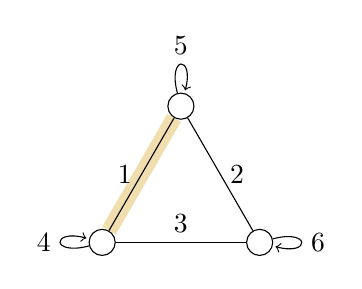
\begin{tikzpicture}
        \node[circle, draw] (1) at (0,0) {};
        \node[circle, draw] (2) at (2,0) {};
        \node[circle, draw] (3) at (1,1.73) {};
        
        \draw (1) --               node[above] {3} (2);
        \draw (2) --               node[right] {2} (3);
        \draw[preaction={draw=darktan, line width=2mm}] 
              (3) --               node[left]  {1} (1);
        \draw (1) edge[loop left]  node        {4} (1);
        \draw (2) edge[loop right] node        {6} (2);
        \draw (3) edge[loop above] node        {5} (3);
    \end{tikzpicture}
    \caption{Agent $a_1$}
  \end{subfigure}
  \hfill
  \begin{subfigure}{0.3\textwidth}
    \centering
    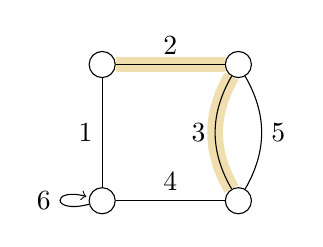
\begin{tikzpicture}
        \node[draw,circle] (r) at (0,0) {};
        \node[draw,circle] (q) at (0,1.73) {};
        \node[draw,circle] (w) at (1.73,1.73) {};
        \node[draw,circle] (t) at (1.73,0) {};

        \draw[preaction={draw=darktan, line width=2mm}] 
        (q) -- node[above] {2} (w);
        \draw
        (q) -- node[left] {1} (r);
        \draw
        (r) -- node[above] {4} (t);
        \path (t) 
        edge [bend left, preaction={draw=darktan, line width=2mm}] 
        node[left] {3} (w);
        \path (t) 
        edge [bend right]
        node[right] {5} (w);
        \path (r) 
        edge [loop left] 
        node[left] {6} (r);
    \end{tikzpicture}
    \caption{Agent $a_2$}
  \end{subfigure}
  \hfill
  \begin{subfigure}{0.3\textwidth}
    \centering
    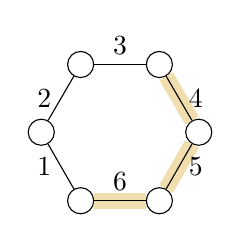
\begin{tikzpicture}        
        \node[draw, circle] (q) at (0,0)       {};
        \node[draw, circle] (w) at (1,0)       {};
        \node[draw, circle] (e) at (1.5,0.87)  {};
        \node[draw, circle] (r) at (1,1.73)    {};
        \node[draw, circle] (t) at (0,1.73)    {};
        \node[draw, circle] (y) at (-0.5,0.87) {};

        % Draw the edges
        \draw[preaction={draw=darktan, line width=2mm}] 
              (q) -- node[above] {6} (w);
        \draw[preaction={draw=darktan, line width=2mm}] 
              (w) -- node[right] {5} (e);
        \draw[preaction={draw=darktan, line width=2mm}] 
              (e) -- node[right] {4} (r);
        \draw (r) -- node[above] {3} (t);
        \draw (t) -- node[left]  {2} (y);
        \draw (y) -- node[left]  {1} (q);
    \end{tikzpicture}
    \caption{Agent $a_3$}
  \end{subfigure}

  \bigskip

  \begin{subfigure}{\textwidth}
    \centering
    \begin{tikzpicture}[scale=1.5]
        \node[draw, circle]                         (1) at (0,0)       {1};
        \node[draw, circle, fill=darktan]           (2) at (1,0)       {2};
        \node[draw, circle, fill=darktan]           (3) at (1.5,0.87)  {3};
        \node[draw, circle, fill=complementaryblue] (4) at (1,1.73)    {4};
        \node[draw, circle, fill=complementaryblue] (5) at (0,1.73)    {5};
        \node[draw, circle, fill=complementaryblue] (6) at (-0.5,0.87) {6};

        \begin{scope}[on background layer]
            \draw[line width=2mm, averagegreen] (2) to (4);
            \draw[line width=2mm, averagegreen] (3) to (4);
        \end{scope}

        \draw[<->] (1) -- (2);
        \draw[<->] (1) -- (3);
        \draw[<-]  (1) -- (4);
        \draw[<->] (2) -- (4);
        \draw[<->] (3) -- (4);
        \draw[<->] (3) -- (5);
        \draw[->]  (5) -- (1);
        \draw[->]  (5) -- (2);
        \draw[->]  (5) -- (3);
        \draw[->]  (6) -- (1);
        \draw[->]  (6) -- (2);
        \draw[->]  (6) -- (3);
        \draw[->]  (6) -- (3);
    \end{tikzpicture}
    \caption{The exchange graph of the allocation}
  \end{subfigure}
  \caption{(a)-(c) shows three agents represented by their valuation matroids, the allocation $A$ highlighted in yellow. (d) shows the exchange graph $D(A)$, with $F_{a_1}$ highlighted in yellow, $S_>$ in blue and the transfer paths in green.}
  \label{fig:not_mms}
\end{figure}

\begin{algorithm}{\pr{AlgMMS}~\cite{barman2021existence}}{mms}
\begin{pseudo}[label=\small\arabic*, indent-mark]
Compute a clean, MAX-USW allocation $A = (A_1,\dots,A_n)$ \\
Initialize $S_< := \{ i\in N : v_i(A_i) < \mu_i \}$ \\
Initialize $S_> := \{ i\in N : v_i(A_i) > \mu_i \}$ \\
\kw{while} $S_<\neq\emptyset$, \kw{do}  \\+
    Select any agent $i \in S_<$\\
    Construct the exchange graph $D(A)$ \\
    Let $F_i := \{ g\in E : \Delta_i(A_i, g) = 1 \}$ \\
    Let $P = (g_1,\dots,g_t)$ be a shortest path $F_i \to \bigcup_{j\in S_>}A_j$ in $D(A)$ \\
    Update $A_k \leftarrow A_k\Lambda P$ for all $k\in N$ \\
    Update $A_i \leftarrow A_i + g_1$ and $A_j \leftarrow A_j - g_t$ \\
    Reset $S_< := \{ i\in N : v_i(A_i) < \mu_i \}$ \\
    Reset $S_> := \{ i\in N : v_i(A_i) > \mu_i \}$ \\-
\kw{end} \\
Let $junk := E \setminus \bigcup_{i=1}^n A_i$ be the set of unallocated goods \\
\kw{return} $(A_1 \cup junk, A_2,\dots,A_n)$
\end{pseudo}
  
\end{algorithm}

In this scenario, we have three agents $a_1, a_2$ and $a_3$ and six goods $E=\{1,\dots,6\}$. The allocation $A$ is highlighted in yellow: $A_{a_1} = \{1\}$, $A_{a_2} = \{2,3\}$ and $A_{a_3} = \{4,5,6\}$. It should be clear that the maximin share of each agent is 2; in the situation depicted, $a_3$ has received a bundle of value 3, at the expense of $a_1$, who only received a bundle of value 1. This might be the initial allocation produced with the matroid union algorithm (it is MAX-USW, as SW$(A) = 6 = |E|$). Since $v_{a_1}(A_{a_1}) = 1 < \mu_{a_1} = 2$, we have $S_<=\{a_1\}$, and need to transfer a good into $A_{a_1}$. However, since none of the goods in $A_{a_3}$ are of value to $a_1$, we need to find a transfer path via some other good.

Figure~\ref{fig:not_mms}(d) shows the exchange graph $D(A)$ (ie. the directed graph with a node per good, and an edge $(u,v)$ iff good $u$ can be exchanged with good $v$ for no loss in value for the current holder of $u$). Highlighted in yellow are the goods in $F_{a_1}$, the set of goods $g$ such that $\Delta_{a_1}(A_{a_1}, g) = 1$. The blue nodes are the goods belonging to an agent in $S_>$, the set of agents who have received more than their MMS. The green edges show the paths between these two sets of goods. As we can see, the available transfer paths are $(2,4)$ and $(3,4)$, representing a transfer of good 4 from $A_{a_3}$ to $A_{a_2}$, and good 2 or 3 from $A_{a_2}$ to $A_{a_1}$, respectively.

\begin{figure}[ht!]
    \begin{subfigure}{0.3\textwidth}
      \centering
      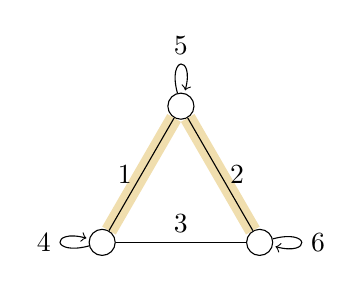
\begin{tikzpicture}
          \node[circle, draw] (1) at (0,0) {};
          \node[circle, draw] (2) at (2,0) {};
          \node[circle, draw] (3) at (1,1.73) {};
          
          \draw (1) --               node[above] {3} (2);
          \draw[preaction={draw=darktan, line width=2mm}]
                (2) --               node[right] {2} (3);
          \draw[preaction={draw=darktan, line width=2mm}] 
                (3) --               node[left]  {1} (1);
          \draw (1) edge[loop left]  node        {4} (1);
          \draw (2) edge[loop right] node        {6} (2);
          \draw (3) edge[loop above] node        {5} (3);
      \end{tikzpicture}
      \caption{Agent $a_1$}
    \end{subfigure}
    \hfill
    \begin{subfigure}{0.3\textwidth}
      \centering
      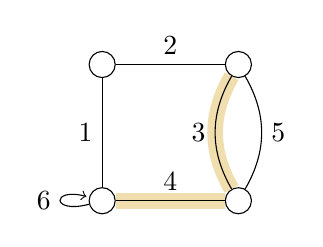
\begin{tikzpicture}
          \node[draw,circle] (r) at (0,0) {};
          \node[draw,circle] (q) at (0,1.73) {};
          \node[draw,circle] (w) at (1.73,1.73) {};
          \node[draw,circle] (t) at (1.73,0) {};
  
          \draw (q) -- node[above] {2} (w);
          \draw (q) -- node[left] {1} (r);
          \draw[preaction={draw=darktan, line width=2mm}] 
                (r) -- node[above] {4} (t);
          \path (t) 
          edge [bend left, preaction={draw=darktan, line width=2mm}] 
          node[left] {3} (w);
          \path (t) 
          edge [bend right]
          node[right] {5} (w);
          \path (r) 
          edge [loop left] 
          node[left] {6} (r);
      \end{tikzpicture}
      \caption{Agent $a_2$}
    \end{subfigure}
    \hfill
    \begin{subfigure}{0.3\textwidth}
      \centering
      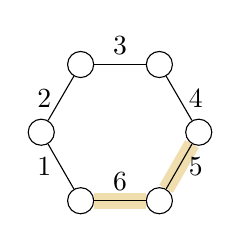
\begin{tikzpicture}        
          \node[draw, circle] (q) at (0,0)       {};
          \node[draw, circle] (w) at (1,0)       {};
          \node[draw, circle] (e) at (1.5,0.87)  {};
          \node[draw, circle] (r) at (1,1.73)    {};
          \node[draw, circle] (t) at (0,1.73)    {};
          \node[draw, circle] (y) at (-0.5,0.87) {};
  
          % Draw the edges
          \draw[preaction={draw=darktan, line width=2mm}] 
                (q) -- node[above] {6} (w);
          \draw[preaction={draw=darktan, line width=2mm}] 
                (w) -- node[right] {5} (e);
          \draw (e) -- node[right] {4} (r);
          \draw (r) -- node[above] {3} (t);
          \draw (t) -- node[left]  {2} (y);
          \draw (y) -- node[left]  {1} (q);
      \end{tikzpicture}
      \caption{Agent $a_3$}
    \end{subfigure}

    \caption{The resulting MMS-fair allocation after augmenting along $(2,4)$.}
    \label{fig:yes_mms}
  \end{figure}

Finally, after all agents have received their MMS, any remaining unallocated goods are simply allocated to agent 1. This ensures that the allocation is complete, though not necessarily clean. These goods, denoted $junk$ in Algorithm~\ref{alg:mms}, are the goods for which no agent has any additional value, either because they were always 0-valued or because every agent has achieved a basis in their matroid.

\pr{AlgMMS} highlights how strong fairness guarantees can be made when working with matroid-rank valuations. In the general, additive case, even computing the MMS of a single agent is NP-hard. With this algorithm, we can produce MMS-fair allocations in polynomial time.


\paragraph{Yankee Swap.}

\section{Matroid partitioning}
\label{sec:matroid-union-impl}
\subsection{Exchange graph}
\subsection{Shortest path}
\subsection{Transfer path augmentation}
\chapter{Fair allocation with binary submodular valuations}
\skelpars[2]

\section{Yankee Swap}
\skelpars[12]

\section{Barman and Verma's MMS algorithm}
\skelpars[9]
\chapter{Fair allocation with matroid constraints}
\skelpars[2]

\section{A very cool algorithm will be discussed here}
\skelpars[12]

\section{This algorithm is okay as well}
\skelpars[8]
\chapter{Results}
\skelpars[24]
\chapter{Discussion}
\label{chap:conclusions}
\skelpar

\section{Limitations}
Little support exists in Julia for working with Multigraphs at the moment.

\section{Future work}
\begin{enumerate}
  \item Exchange graphs, shortest path, augmentation. Stop recalculating everything after a transfer. Keep track of shortest paths, most will not change.
  \item Parallelization?
  \item Eliciting actual user preferences as matroids
\end{enumerate}

\section{Concluding remarks}
Initially, all I knew about this thesis was that it was going to have something to do with fair allocation. Looking around for recent allocation algorithms, the study of which might form part of a thesis, Viswanathan and Zick's Yankee Swap algorithm caught my attention. By restricting the valuations to the class of matroid rank functions, a seemingly simple algorithm could deliver extraordinarily well on a range of fairness objectives intractable in the general, additive case. My interest piqued, I wanted to understand how it worked, and set about implementing the algorithm using Hummel and Hetland's Allocations.jl library. Almost immediately I was flummoxed by how to represent the matroid rank valuations. I had assumed that there would exist some library to facilitate working programmatically with matroids, similar to how Graphs.jl enables working with graphs without needing to reinvent the wheel graph. At the time I was unable to find any such library, and so the research question for this thesis came to be: how might one design and implement a Julia library to support the implementation of and experimentation with matroidal fair allocation algorithms? 

The primary goal of this thesis was to build Matroids.jl as an answer to that question---a practical tool to complement the theoretical toolkit provided by matroid theory. An important sub-goal was to figure out how to make Matroids.jl performant; as we have seen, matroids permit many powerful polynomial-time operations, such as the matroid partition algorithm, that papers on matroidal fair allocation algorithms use in their analyses to show that allocations can be found efficiently. This obscures many implementation-level optimization decisions that can drastically improve the practical runtime of the implemented algorithms. One example of such an optimization is to use the rank function as sparingly as possible, in favor of cheaper independence or cardinality checks, as I discuss when giving some algorithm implementations in Chapter~\ref{chap:yankee-swap}.

Late in the project, I realized that there does in fact exist matroid libraries in Julia, in all likelihood vastly more performant and feature-rich than Matroids.jl would ever be\footnote{See for instance \href{https://docs.oscar-system.org/stable/Combinatorics/matroids/}{https://docs.oscar-system.org/stable/Combinatorics/matroids/}.}. The primary target demographic for Matroids.jl had always been fair allocation researchers, but upon witnessing the capabilities of my more advanced competitors, a secondary target demographic came to the fore, namely students, computer programmers and non-mathematicians such as myself. All along, I realized, I had been building the library for myself, the library that I had needed when I wanted to figure out how Yankee Swap worked, which was a simple-to-use matroid library that only concerned itself with the most basic aspects of matroids as they related to fair  allocation.

While matroid theory might seem an extremely abstract and niche subfield of mathematics, it has found applicability in the field of fair allocation, which in the end deals with problems of a highly practical and everyday nature. The aim of fair allocation, to deliver provably fair mechanisms for the distribution of resources, is a noble goal, and if a problem permits a matroidal representation, it can utilize algorithms that deliver very well indeed. If Matroids.jl is able to serve as a soft introduction to matroid theory for a computer programmer interested in understanding fair allocation algorithms, and if that computer programmer goes on to build a real-world solution for fair allocation, then Matroids.jl has achieved its goals as far as I am concerned.


\printskelnotes{}
\bibliographystyle{alpha}
\bibliography{refs}








\begin{appendices}


% \chapter{Tables}

% \begin{table*}[ht]
%   \centering
%   \caption{Observed mean values for \pr{Random-Knuth-Matroid}.}
%   \label{tab:coarsening}
%   \begin{threeparttable}
%     \begin{tabular}{llllllllll}
%       \toprule
%       $n$ & $(p_1, p_2, \ldots)$ & Trials                  & Bases & $|F_2|$ & $|F_3|$ & $|F_4|$ & $|F_5|$ & $|F_6|$ \\
%       \midrule
%       10  & $(6, 0, 0)$          & 44 \textsuperscript{a}  & 100.0 & 30.3    & 1.0     &         &         &         \\
%       10  & $(6, 0, 0)$          & 917 \textsuperscript{b} & 76.6  & 28.3    & 25.5    & 1.0     &         &         \\
%       10  & $(6, 0, 0)$          & 39 \textsuperscript{c}  & 51.6  & 31.0    & 38.5    & 27.8    & 1.0     &         \\
%       10  & $(5, 1, 0)$          & 26 \textsuperscript{a}  & 107.2 & 33.3    & 1.0     &         &         &         \\
%       10  & $(5, 1, 0)$          & 935 \textsuperscript{b} & 102.6 & 32.7    & 33.0    & 1.0     &         &         \\
%       10  & $(5, 1, 0)$          & 39 \textsuperscript{c}  & 53.0  & 33.0    & 44.6    & 48.0    & 1.0     &         \\
%       10  & $(5, 2, 0)$          & 791 \textsuperscript{a} & 108.0 & 32.5    & 1.0     &         &         &         \\
%       10  & $(5, 2, 0)$          & 201 \textsuperscript{b} & 100.0 & 32.9    & 32.6    & 1.0     &         &         \\
%       10  & $(5, 2, 0)$          & 8 \textsuperscript{c}   & 24.6  & 30.1    & 39.9    & 66.0    & 1.0     &         \\
%       10  & $(6, 1, 0)$          & 862 \textsuperscript{a} & 99.2  & 28.4    & 1.0     &         &         &         \\
%       10  & $(6, 1, 0)$          & 137 \textsuperscript{b} & 69.8  & 28.1    & 29.1    & 1.0     &         &         \\
%       10  & $(6, 1, 0)$          & 1 \textsuperscript{c}   & 48.0  & 33.0    & 41.0    & 33.0    & 1.0     &         \\
%       10  & $(4, 2, 0)$          & 12 \textsuperscript{a}  & 111.1 & 36.3    & 1.0     &         &         &         \\
%       10  & $(4, 2, 0)$          & 950 \textsuperscript{b} & 119.2 & 35.9    & 42.5    & 1.0     &         &         \\
%       10  & $(4, 2, 0)$          & 38 \textsuperscript{c}  & 73.4  & 36.4    & 52.6    & 39.4    & 1.0     &         \\
%       10  & $(3, 3, 0)$          & 4 \textsuperscript{a}   & 115.0 & 39.0    & 1.0     &         &         &         \\
%       10  & $(3, 3, 0)$          & 911 \textsuperscript{b} & 138.0 & 38.5    & 53.3    & 1.0     &         &         \\
%       10  & $(3, 3, 0)$          & 85 \textsuperscript{c}  & 90.6  & 38.7    & 61.9    & 36.2    & 1.0     &         \\
%       10  & $(0, 6, 0)$          & 767 \textsuperscript{b} & 171.8 & 45.0    & 85.6    & 1.0     &         &         \\
%       10  & $(0, 6, 0)$          & 230 \textsuperscript{c} & 128.4 & 45.0    & 95.8    & 72.7    & 1.0     &         \\
%       10  & $(0, 6, 0)$          & 3 \textsuperscript{d}   & 52.3  & 45.0    & 94.7    & 90.3    & 32.7    & 1.0     \\
%       % 10  & $(0, 1, 1, 1)$       & 3 \textsuperscript{d}   & 52.3  & 45.0    & 94.7    & 90.3    & 32.7    & 1.0     &         &         \\
%       \bottomrule\addlinespace[1ex]
%     \end{tabular}
%     \begin{tablenotes}\footnotesize
%       \item [a] Averages for experiments when final rank was 3.
%       \item [b] Averages for experiments when final rank was 4.
%       \item [c] Averages for experiments when final rank was 5.
%       \item [d] Averages for experiments when final rank was 6.
%     \end{tablenotes}
%   \end{threeparttable}
% \end{table*}


\chapter{Code snippets}

\section{\texorpdfstring{$\texttt{random\_kmc\_v1}$}{random\_kmc\_v1}}
\label{apx:randkmcv1}
\jlinputlisting{random_kmc_v1.jl}

\section{\texorpdfstring{\mono{random\_kmc\_v2} and \mono{random\_kmc\_v3}}{random\_kmc\_v2 and random\_kmc\_v3}}
\label{apx:randkmcv2}
\jlinputlisting{random_kmc_v2.jl}

\section{\texorpdfstring{$\texttt{random\_kmc\_v4}$}{random\_kmc\_v4}}
\label{apx:randkmcv4}
\jlinputlisting{random_kmc_v4.jl}

\section{\texorpdfstring{$\texttt{random\_kmc\_v5}$}{random\_kmc\_v5}}
\label{apx:randkmcv5}
\jlinputlisting{random_kmc_v5.jl}

\section{\texorpdfstring{$\texttt{random\_kmc\_v6}$}{random\_kmc\_v6}}
\label{apx:randkmcv6}
\jlinputlisting{random_kmc_v6.jl}


\end{appendices}

\end{document}